\documentclass[twoside,11pt]{article}

% Any additional packages needed should be included after jmlr2e.
% Note that jmlr2e.sty includes epsfig, amssymb, natbib and graphicx,
% and defines many common macros, such as 'proof' and 'example'.
%
% It also sets the bibliographystyle to plainnat; for more information on
% natbib citation styles, see the natbib documentation, a copy of which
% is archived at http://www.jmlr.org/format/natbib.pdf

\usepackage{jmlr2e}
\usepackage{doi}

\usepackage{subcaption}
\usepackage{url}
\usepackage{color}
\usepackage{listings}
\usepackage{amsmath}
\usepackage{tikz}
\usetikzlibrary{bayesnet}

% Definitions of handy macros can go here

% Heading arguments are {volume}{year}{pages}{submitted}{published}{author-full-names}

\jmlrheading{?}{2015}{?-?}{?/??}{?/??}{Jaakko Luttinen}

% Short headings should be running head and authors last names

\ShortHeadings{BayesPy: Variational Bayesian Inference in Python}{Luttinen}
\firstpageno{1}

\lstset{ %
  basicstyle=\footnotesize,        % the size of the fonts that are used for the code
  breakatwhitespace=false,         % sets if automatic breaks should only happen at whitespace
  breaklines=true,                 % sets automatic line breaking
  captionpos=b,                    % sets the caption-position to bottom
  commentstyle=\color{green},    % comment style
  deletekeywords={...},            % if you want to delete keywords from the given language
  escapeinside={\%*}{*)},          % if you want to add LaTeX within your code
  extendedchars=true,              % lets you use non-ASCII characters; for 8-bits encodings only, does not work with UTF-8
%  frame=single,                    % adds a frame around the code
  keepspaces=true,                 % keeps spaces in text, useful for keeping indentation of code (possibly needs columns=flexible)
  keywordstyle=\color{blue},       % keyword style
  morekeywords={*,...},            % if you want to add more keywords to the set
  firstnumber=last,
  numbers=left,                    % where to put the line-numbers; possible values are (none, left, right)
  numbersep=10pt,                   % how far the line-numbers are from the code
  numberstyle=\tiny\color{black}, % the style that is used for the line-numbers
  rulecolor=\color{black},         % if not set, the frame-color may be changed on line-breaks within not-black text (e.g. comments (green here))
  showspaces=false,                % show spaces everywhere adding particular underscores; it overrides 'showstringspaces'
  showstringspaces=false,          % underline spaces within strings only
  showtabs=false,                  % show tabs within strings adding particular underscores
  stepnumber=1,                    % the step between two line-numbers. If it's 1, each line will be numbered
  stringstyle=\color{orange},     % string literal style
  tabsize=2,                       % sets default tabsize to 2 spaces
%  title=\lstname,                   % show the filename of files included with \lstinputlisting; also try caption instead of title
  belowcaptionskip=1\baselineskip,
  breaklines=true,
  frame=L,
  xleftmargin=1.3\parindent,
  showstringspaces=false,
  basicstyle=\footnotesize\ttfamily,
%  keywordstyle=\bfseries\color{green!40!black},
%  commentstyle=\itshape\color{purple!40!black},
%  identifierstyle=\color{blue},
%  stringstyle=\color{orange},
  language=Python
}


\begin{document}

\title{BayesPy: Variational Bayesian Inference in Python}

\author{\name Jaakko Luttinen \email jaakko.luttinen@aalto.fi \\
       \addr Department of Computer Science\\
       Aalto University, Finland}

\editor{?}

\maketitle

\begin{abstract}%   <- trailing '%' for backward compatibility of .sty file
  BayesPy is an open-source Python software package for performing variational
  Bayesian inference.  It is based on the variational message passing framework
  and supports conjugate exponential family models.  By removing the tedious
  task of implementing the variational Bayesian update equations, the user can
  construct models faster and in a less error-prone way.  Simple syntax,
  flexible model construction and efficient inference make BayesPy suitable for
  both average and expert Bayesian users.
\end{abstract}

\begin{keywords}
  Variational Bayes, variational message passing, Python, probabilistic
  programming
\end{keywords}

\section{Introduction}

Bayesian framework provides a theoretically solid and consistent way to
construct models and perform inference.  In practice, however, the inference is
usually analytically intractable and is therefore based on approximation methods
such as variational Bayes (VB), expectation propagation (EP) and Markov chain
Monte Carlo (MCMC) \citep{Bishop:2006}.  Deriving and implementing the formulas
for an approximation method is often straightforward but tedious, time consuming
and error prone.


BayesPy is a Python 3 package providing tools for constructing models and
performing VB inference easily and efficiently.  It is based on the variational
message passing (VMP) framework which defines a simple message passing protocol
\citep{Winn:2005}.  This enables implementation of small general nodes that can
be used as building blocks for large complex models.  BayesPy offers a
comprehensive collection of built-in nodes that can be used to build a wide
range of models and a simple interface for implementing custom nodes.  The
package is released under the GNU General Public License v3.0 (GPLv3).


Several other projects have similar goals for making Bayesian inference easier
and faster to apply.  VB inference is available in Bayes Blocks
\citep{Raiko:2007}, VIBES \citep{Bishop:2002} and Infer.NET \citep{Infer.NET}.
Bayes Blocks is an open-source C++/Python package but limited to scalar Gaussian
nodes and a few deterministic functions, thus making it very limited.  VIBES is
an old software package for Java, released under the revised BSD license, but it
is no longer actively developed.  VIBES has been replaced by Infer.NET, which
%supports a wide range of posterior approximations.  However, Infer.NET
is partly closed source and licensed for non-commercial use only.  Instead of VB
inference, mainly MCMC is supported by other projects such as PyMC \citep{PyMC},
OpenBUGS \citep{OpenBUGS}, Dimple \citep{Dimple} and Stan \citep{Stan}.  Thus,
there is a need for an open source and maintained VB software package.



\section{Features}


BayesPy can be used to construct conjugate exponential family models.  The
documentation provides detailed examples of how to construct, for instance,
principal component analysis models, linear state-space models, mixture models
and hidden Markov models.  In addition, BayesPy has been used in two
publications about parameter expansion and time-varying dynamics for linear
state-space models \citep{Luttinen:2013,Luttinen:2014}.
% , which show that it is applicable to large complex models requiring efficient
% inference.



Using BayesPy for Bayesian inference consists of four main steps: constructing
the model, providing data, finding the posterior approximation and examining the
results.  The user constructs the model from small modular blocks called nodes.
Roughly, each node corresponds to a latent variable, a set of observations or a
deterministic function.
%Some of the nodes may be set as observed by providing
%data.
The inference engine is used to run the message passing algorithm in order to
obtain the posterior approximation.  The resulting posterior can be examined,
for instance, by using a few built-in plotting functions or printing the
parameters of the posterior distributions.


Nodes are the key part of BayesPy as they are used to construct the model.
There are two types of nodes in BayesPy: stochastic and deterministic.
Stochastic nodes correspond to probability distributions and deterministic nodes
correspond to functions.  Built-in stochastic nodes include all common
exponential family distributions (e.g., Gaussian, gamma and Dirichlet
distributions), a general mixture distribution and a few complex nodes for
dynamic variables (e.g., discrete and Gaussian Markov chains).  Built-in
deterministic nodes include a gating node and a general sum-product node.
%The
%documentation also provides instructions for implementing new nodes in case the
%built-in collection is insufficient.
In case a model cannot be constructed using the built-in nodes, the
documentation provides instructions for implementing new nodes.



BayesPy is designed to be simple enough for average users but flexible and
efficient enough for expert users.  One goal is to keep the syntax easy and
intuitive to read and write by making it similar to the mathematical formulation
of the model.  Missing values are easy to handle and the variables can be
monitored by plotting the posterior distributions during the learning.  BayesPy
has also preliminary support for some advanced VB methods such as stochastic
variational inference \citep{Hoffman:2013}, deterministic annealing
\citep{Katahira:2008}, collapsed inference \citep{Hensman:2012},
Riemannian-gradient-based optimization \citep{Honkela:2010}, parameter
expansions \citep{Qi:2007} and pattern searches \citep{Honkela:2003}.  For
developers, the unit testing framework helps in finding bugs, making changes and
implementing new features in a robust manner.



BayesPy can be installed similarly to other Python packages.  It requires Python
3 and a few popular packages: NumPy, SciPy, matplotlib and h5py.  The latest
release can be installed from Python Package Index (PyPI) and detailed
instructions can be found from the comprehensive online documentation
\citep{bayespy.org}.  The latest development version is available at
GitHub\footnote{\url{https://github.com/bayespy/bayespy}}, which is also the
platform used for reporting bugs and making pull requests.


%- numpy, scipy, matplotlib, h5py

%- documentation

%- installation

%- repository


%- clear syntax

%- unit tests

%- parameter expansion

%- monitoring

%- missing values

%- examples: PCA, LSSM, HMM, mixture models

%- used in two publications, \citep{Luttinen:2013, Luttinen:2014}


\section{Example}

This section demonstrates BayesPy with a Gaussian mixture model.  A simple
artificial dataset is created by drawing 200 samples from a 2-dimensional
Gaussian distribution.  80 samples have mean $[1, 1]$ and 120 samples have mean
$[0, 0]$:
\begin{lstlisting}
import numpy as np
N = 200, D = 2
data = np.random.randn(N, D)
data[:80,:] += np.ones(D)
\end{lstlisting}
We construct a mixture model for the data and assume that the parameters, the
cluster assignments and the true number of clusters are unknown.  The model uses
a maximum number of five clusters but the effective number of clusters will be
determined automatically:
\begin{lstlisting}
K = 5
\end{lstlisting}
The unknown cluster means and precision matrices are given Gaussian and Wishart
prior distributions:
\begin{lstlisting}
from bayespy import nodes
mu = nodes.Gaussian(np.zeros(D), 0.01*np.identity(D), plates=(K,))
Lambda = nodes.Wishart(D, 0.01*np.identity(D), plates=(K,))
\end{lstlisting}
The \texttt{plates} keyword argument is used to define repetitions similarly as
the plate notation in graphical models.  The cluster assignments are categorical
variables, and the cluster probabilities are given a Dirichlet prior
distribution:
\begin{lstlisting}
alpha = nodes.Dirichlet(0.01*np.ones(K))
z = nodes.Categorical(alpha, plates=(N,))
\end{lstlisting}
The observations are from a Gaussian mixture distribution:
\begin{lstlisting}
y = nodes.Mixture(Z, nodes.Gaussian, mu, Lambda)
\end{lstlisting}
The second argument for the \texttt{Mixture} node defines the type of the
mixture distribution, in this case Gaussian.  The variable is marked as observed
by providing the data:
\begin{lstlisting}
y.observe(data)
\end{lstlisting}
Next, we want to find the posterior approximation for our latent variables.  We
create the variational Bayesian inference engine:
\begin{lstlisting}
from bayespy.inference import VB
Q = VB(y, mu, z, Lambda, alpha)
\end{lstlisting}
Before running the VMP algorithm, the symmetry in the model is broken by
a random initialization of the cluster assignments:
\begin{lstlisting}
z.initialize_from_random()
\end{lstlisting}
Without the random initialization, the clusters would not be separated.  The VMP
algorithm is run for 100 iterations or until convergence:
\begin{lstlisting}
Q.update(repeat=100)
\end{lstlisting}
The results can be examined, for instance, by printing the posterior
distributions of some variables:
\begin{lstlisting}
print(alpha)
print(mu)
\end{lstlisting}
In addition, module \texttt{bayespy.plot} contains several plotting functions to
examine the results visually.


\section{Comparison with Infer.NET}


This section provides a brief comparison with Infer.NET because it is another
active project implementing the variational message passing algorithm, whereas
the other related active projects implement MCMC.  The main advantages of
Infer.NET over BayesPy are its support for non-conjugate models and other
inference engines.  On the other hand, BayesPy is open-source software and
supports several advanced VB methods (e.g., stochastic variational inference and
collapsed inference).


The speed of the packages were compared by using two widely used models: a
Gaussian mixture model (GMM) and principal component analysis
(PCA).\footnote{The scripts for running the experiments are available in the
  supplementary material.}  Both models were run for small and large
artificially generated datasets.  For GMM, the small model used 10 clusters for
200 observations with 2 dimensions, and the large model used 40 clusters for
2000 observations with 10 dimensions.  For PCA, the small model used
10-dimensional latent space for 500 observations with 20 dimensions, and the
large model used 40-dimensional latent space for 2000 observations with 100
dimensions.  Infer.NET used a fully factorizing approximation for the PCA model,
whereas BayesPy did not factorize with respect to the latent space dimensions.
The experiments were run on a Linux computer with a quad-core processor
(i7-4702MQ).  Because the packages run practically identical algorithms and thus
converged to similar solutions in a similar number of iterations (50--100
iterations depending on the dataset), we compare the average CPU time per
iteration.


The results are summarized in Table~\ref{tab:speed}.  On the smaller datasets,
Infer.NET is slightly faster because BayesPy has some overhead of Python.
However, on the larger datasets, BayesPy is significantly faster because it uses
BLAS and LAPACK libraries for fast numerical operations.\footnote{Assuming that
  NumPy uses BLAS/LAPACK because BayesPy uses NumPy for numerical operations.}
In addition, if using multi-threaded BLAS and LAPACK, the difference in
wall-clock time can be even larger than in CPU time.  The speed of BayesPy for
these models could potentially be improved by using collapsed or stochastic
variational inference, and the accuracy could be improved by using
Gaussian-Wishart nodes which do not factorize with respect to the Gaussian and
Wishart variables.

\begin{table}[tb]
  \centering
  \caption{The average CPU time (in milliseconds) per iteration for each dataset.}
  \small
  \begin{tabular}{ccccc}
    &
    Small GMM
    &
    Large GMM
    &
    Small PCA
    &
    Large PCA
    \\
    \hline
    BayesPy     & 45 & 210  & 52 & 380
    \\
    Infer.NET   & 26 & 4400 & 37 & 2200
  \end{tabular}
  \label{tab:speed}
\end{table}


% related active software projects discussed in the introduction,

% Because the other
% active Bayesian software packages discussed in the introduction do not implement
% the variational message passing algorithm,

%* compiled

%* non-conjugate

%* other engines

%* open source

%* advanced


%* dynamic nodes

% \begin{figure}
%   \centering
%   \begin{tikzpicture}
%     \node [obs] (yn) {$y_n$};
%     \node [latent, above left=of yn] (mu) {$\mu$};
%     \node [latent, above right=of yn] (tau) {$\tau$};

%     \edge {mu, tau} {yn};

%     \tikzstyle{plate caption} = [caption, node distance=0, inner sep=0pt,
%     below=5pt of #1.south]

%     \plate {} {(yn)} {$n=1,\ldots,10$};
%   \end{tikzpicture}
%   \caption{Graphical model of the example problem.}
%   \label{fig:graphical_model}
% \end{figure}
% In order to demonstrate BayesPy, this section solves an extremely simple problem
% but which includes the main steps of using BayesPy.  The task is to estimate the
% unknown mean and precision parameters of a Gaussian distribution given ten
% observations.  Thus, the likelihood function is Gaussian:
% \begin{align*}
%   p(y_1,\ldots,y_{10}|\mu,\tau) &= \prod^{10}_{n=1}\mathcal{N}(y_n | \mu, \tau),
% \end{align*}
% where the Gaussian distribution is parameterized by precision instead of
% variance.  The unknown mean $\mu$ and precision $\tau$ are given broad Gaussian
% and gamma priors, respectively:
% \begin{align*}
%   p(\mu) &= \mathcal{N}(\mu|0, 10^{-6}), & p(\tau) &= \mathcal{G}(\tau|10^{-6},
%   10^{-6}).
% \end{align*}
% Figure~\ref{fig:graphical_model} shows the graphical model of this simple model.
% The model is constructed in BayesPy by creating nodes:
% \begin{lstlisting}
% from bayespy.nodes import GaussianARD, Gamma
% mu = GaussianARD(0, 1e-6)
% tau = Gamma(1e-6, 1e-6)
% \end{lstlisting}
% These two nodes represent the two unknown variables that we are interested in.
% They are the parameters of the Gaussian distribution of the observed variable:
% \begin{lstlisting}
% y = GaussianARD(mu, tau, plates=(10,))
% \end{lstlisting}
% The number of observations is given as plates which define the number of
% repetitions.  Note that the syntax of the model construction is similar to the
% mathematical formulation which defines the conditional distributions for each
% variable.  Thus, it is easy to understand the model from the Python code.  After
% the model has been constructed, some nodes are marked as observed and given
% data:
% \begin{lstlisting}
% y.observe([4.5, 3.9, 6.3, 5.6, 4.9, 2.8, 7.4, 6.1, 4.8, 2.1])
% \end{lstlisting}
% Next, we want to find the posterior approximation for our latent variables.  We
% create the VB inference engine:
% \begin{lstlisting}
% from bayespy.inference import VB
% Q = VB(y, mu, tau)
% \end{lstlisting}
% The inference engine takes all the stochastic nodes of the model as input.  The
% message passing algorithm can be run by calling \texttt{update} method:
% \begin{lstlisting}
% Q.update(repeat=100)
% \end{lstlisting}
% The algorithm is run for 100 iterations or until it converges.  In this case,
% the algorithm converges in four iterations.  The posterior approximation can be
% examined, for instance, by plotting the probability density functions of the
% latent variables:
% \begin{lstlisting}
% import bayespy.plot as bpplt
% import numpy as np
% bpplt.pyplot.figure()
% bpplt.pdf(Q[mu], np.linspace(0, 10, num=300))
% bpplt.pyplot.figure()
% bpplt.pdf(Q[tau], np.linspace(0, 2, num=300))
% bpplt.pyplot.show()
% \end{lstlisting}
% Figure~\ref{fig:posterior} shows the resulting approximate posterior
% distributions.  The module \texttt{bayespy.plot} contains functions for simple
% plotting tasks, such as plotting the probability density function or the Hinton
% diagram of a variable.  Note that the standard \texttt{pyplot} module of
% Matplotlib is available at the \texttt{plot} module of BayesPy.
% \begin{figure}
%   \begin{center}
%     \begin{subfigure}[b]{0.4\textwidth}
%       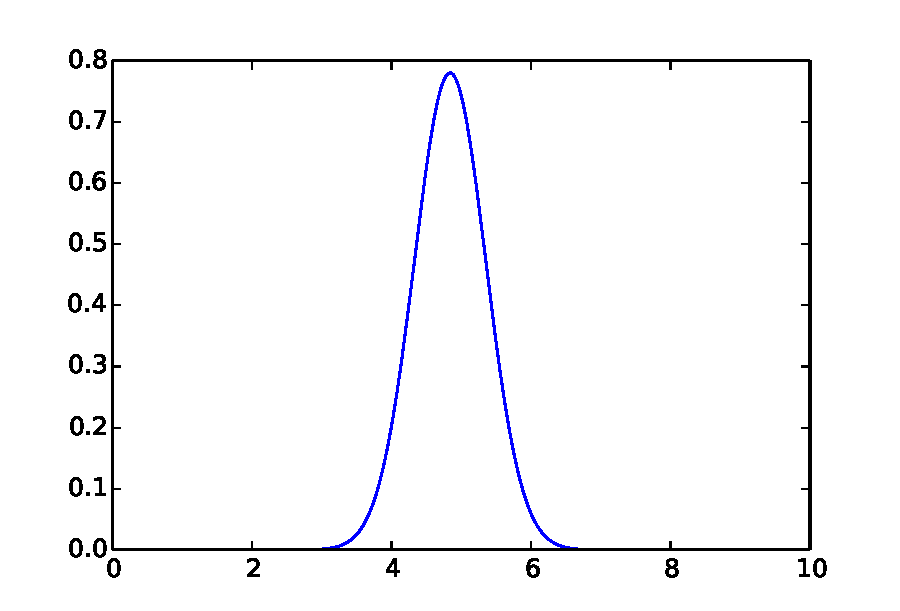
\includegraphics[width=\textwidth]{fig_mu}
%       \caption{$q(\mu)$}
%     \end{subfigure}
%     \begin{subfigure}[b]{0.4\textwidth}
%       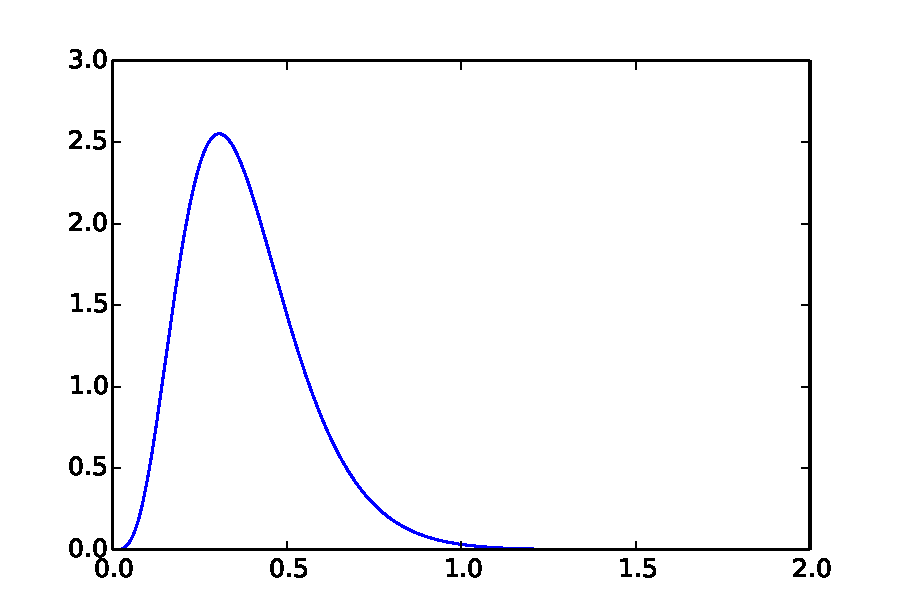
\includegraphics[width=\textwidth]{fig_tau}
%       \caption{$q(\tau)$}
%     \end{subfigure}
%   \end{center}
%   \caption{The posterior approximations of $\mu$ and $\tau$.}
%   \label{fig:posterior}
% \end{figure}

\section{Conclusions}

BayesPy provides a simple and efficient way to construct conjugate exponential
family models and to find the variational Bayesian posterior approximation in
Python.
%
In addition to the standard variational message passing, it supports several
advanced methods such as stochastic and collapsed variational inference.  Future
plans include support for non-conjugate models and non-parametric nodes (e.g.,
Gaussian and Dirichlet processes).
% Future plans for BayesPy include implementing more inference engines (e.g.,
% maximum likelihood, expectation propagation and Gibbs sampling), improving the
% VB engine (e.g., collapsed variational inference \citep{Hensman:2012} and
% Riemannian conjugate gradient method \citep{Honkela:2010}) and implementing nodes
% for non-parametric models (e.g., Gaussian processes and Dirichlet processes).




% Acknowledgements should go at the end, before appendices and references

%\acks{?}


\vskip 0.2in
\bibliography{bibliography/bibliography.bib}

\end{document}

%%% Local Variables: 
%%% mode: latex
%%% TeX-PDF-mode: t
%%% TeX-master: t
%%% End: 
